% Template for PLoS
% Version 1.0 January 2009
%
% To compile to pdf, run:
% latex plos.template
% bibtex plos.template
% latex plos.template
% latex plos.template
% dvipdf plos.template

\documentclass[10pt]{article}

% amsmath package, useful for mathematical formulas
\usepackage{amsmath}
% amssymb package, useful for mathematical symbols
\usepackage{amssymb}

% graphicx package, useful for including eps and pdf graphics
% include graphics with the command \includegraphics
\usepackage{graphicx}

% cite package, to clean up citations in the main text. Do not remove.
\usepackage{cite}

\usepackage{color}

% TODO temporary
\usepackage{todonotes}

% Use doublespacing - comment out for single spacing
%\usepackage{setspace}
%\doublespacing


% Text layout
\topmargin 0.0cm
\oddsidemargin 0.5cm
\evensidemargin 0.5cm
\textwidth 16cm
\textheight 21cm

% Bold the 'Figure #' in the caption and separate it with a period
% Captions will be left justified
\usepackage[labelfont=bf,labelsep=period,justification=raggedright]{caption}

% Use the PLoS provided bibtex style
\bibliographystyle{plos2009}

% Remove brackets from numbering in List of References
\makeatletter
\renewcommand{\@biblabel}[1]{\quad#1.}
\makeatother


% Leave date blank
\date{}

\pagestyle{myheadings}
%% ** EDIT HERE **


%% ** EDIT HERE **
%% PLEASE INCLUDE ALL MACROS BELOW

%% END MACROS SECTION

\begin{document}

% Title must be 150 characters or less
\begin{flushleft}
{\Large
\textbf{Object oriented implementation of Yeadon's human inertial model}
}
% Insert Author names, affiliations and corresponding author email.
\\
Christopher Dembia$^{1,\ast}$,
Jason K. Moore$^{2}$,
Mont Hubbard$^{3}$
\\
\bf{1} Mechanical Engineering, Stanford University, Palo Alto, California, USA
\\
\bf{2} Mechanical Engineering, Cleveland State Universit, Cleveland, Ohio, USA
\\
\bf{3} Mechanical and Aerospace Engineering, University of California, Davis, California, USA
\\
$\ast$ E-mail: Corresponding cld72@cornell.edu
\end{flushleft}

% Please keep the abstract between 250 and 300 words
\section*{Abstract}
Herein we present an open source software implementation of a popular
mathematical method developed by M.R. Yeadon for estimating the body segment
parameters of a human body~\cite{Yeadon1990f}. The software is written in a
high level open source language and provides three interfaces for manipulating
the data and the model including a Python API, text user interface, and a
graphical user interface. Once the human subject measurement data is collected
and provided as an input the software can fit into various data processing
pipelines.
% Please keep the Author Summary between 150 and 200 words
% Use first person. PLoS ONE authors please skip this step.
% Author Summary not valid for PLoS ONE submissions.
%\section*{Author Summary}

\section*{Introduction}
For dynamic analyses, it is typical to treat the human body as a collection of
linked rigid bodies. For accurate simulation and analysis the inertial
properties (mass, center of mass, and moment of inertia) of the body segments
must be estimated. Human mass, center of mass, and inertial properties have
been measured and estimated in a multitude of ways. Each method has its
advantages and disadvantages. Many methods exist including cadaver measurements
(\cite{Dempster1955}, \cite{Clauser1969}, \cite{Chandler1975}), photogrammetry,
ray scanning techniques (\cite{Zatsiorsky1983}, \cite{Zatsiorsky1990}), water
displacement (\cite{Park1999}), rotating platforms (\cite{Griffiths2005}), and
geometrical estimation of the body segments (\cite{Yeadon1990c}).
Bjornstrup \cite{Bjornstrup1995} gives a detailed overview of mostly invasive
methods up to 1995.

\todo[inline]{ Maybe cite de Leva 1999 as a popular one. These citations are
endless though...}

\todo[inline]{Need to cite ``reasonable estimates'' below. Who says this?}

Yeadon's mathematical method is quite attractive as it requires only a set of
simple measurements from a human and provides reasonable estimates of the
individual human's body segment parameters. Furthermore, it is based off of
simple computations and can easily be programmed to provide a quick estimate of
body segment parameters. Yeadon himself developed a Fortran program called ISEG
for his doctoral work \cite{Yeadon1984a} to rapidly compute his inertia model.
The source code is available through the dissertation under the Creative
Commons Attribution-NonCommercial-NoDerivs 2.5 license but is less than
adaptable for inclusion in modern software packages for easy configuration and
visualization.

We make use of Yeadon's model extensively in our dynamics research and
developed a modern object oriented program under a permissive license that
allows for easy inclusion into software packages and includes a graphical user
interface for ease of end user use.

\section*{Yeadon's model}

In 1990 Yeadon published a four-paper series on the subject of simulating
human aerial movement, particularly twisting somersalts. His first paper
\cite{Yeadon1990c} describes a method for obtaining joint angles from film
data, and accordingly delves into how he defines the orientation of the whole
body and the relative orientation of parts of the body. His second paper
\cite{Yeadon1990f} describes in detail the geometry of his human model. He
leaves the description of the model's configuration to his third paper
\cite{Yeadon1990e}, which also details the analytical calculation of the
model's angular momentum. The last paper in the series \cite{Yeadon1990d}
compares the trajectory of an aerial flight between a film recording and a
computer simulation using the model developed in the first 3 papers.

Yeadon provides a lucid explanation of his human inertia model in the series
described above. In this section, we merely seek to summarize his work. The
model is defined in terms of \emph{segments}, \emph{levels}, and \emph{solids}.
These three elements of the model are all shown in Figure \ref{fig:meas}. Note
that we are not concerned with the angular momentum of the model; we are solely
interested in the model's inertial properties.

\begin{description}
    \item[Segments]
        The human is composed of 11 segments. Each of the 4 limbs is composed
        of 2 segments, and the remainder of the body is composed of 3 segments.
        Each of these segments are rigid bodies, but have at least one
        rotational degree of freedom with respect to the segment to which they
        are attached. The segments are labeled as \textbf{C}, \textbf{A1}, and
        so forth.
    \item[Levels]
        Each segment is defined by a series of parallel transverse cross sections.
        These cross sections are referred to as levels, both in
        Yeadon's work and in ours. The model contains a toal of 45 levels.
        Levels are labeled as \textbf{Ls0}, \textbf{La0}, and so forth.  Each
        level is in the shape of a \emph{stadium} (see Figure
        \ref{fig:stadium}). There are a number of exceptions in which the
        stadium degenerates into a circle. We can define a stadium by any 2 of
        the following 5 attributes: its perimeter $p$, radius $r$, thickness
        $t$, width $w$, and depth $d$. The choice of which 2 attributes are
        used to define a given stadium depends on the stadium's location in the
        body, as, for example, it is difficult to measure a perimeter about the
        shoulders (\textbf{Ls4}) so a depth is used instead.
    \item[Solids]
        The inertial properties of each segment are computed by viewing each
        segment as a solid lofted through all the levels in the segment. This
        defines $N-1$ solids in a segment defined by $N$ levels. The solids are
        labeled as \textbf{s0}, \textbf{a0}, and so forth. All solids in a
        segment share the same longitudinal axis. A given solid is
        defined by its two bounding stadia and the longitudinal distance
        between them (the solid's height). These stadium-bounded solids are
        termed \emph{stadium solids}. The only exception is \textbf{s7}, the
        solid above the ear, which is a semi-ellipsoid. The model contains a
        total of 40 solids.  Note that in this formulation we start numbering
        the segments from 0 \footnote{This is to match the Python 0 based
        indexing patterns}, while Yeadon starts numbering the solids from 1.
\end{description}

A key feature of this inertia model is that it can be personalized to a given
individual for subject specifity, though we have not yet discussed this. The
model is personalized via 95 anthropometric measurements. These measurements
serve to define each stadium, and to provide the distance between the stadia
(the heights of the stadium solids).

Much of the utility of the model comes from being able to specify the
configuration of the human in which one desires its inertial properties. The
configuration is specified via 21 joint angles between the various segments,
all of which are labeled in Figure \ref{fig:config}.

Thus, Yeadon's model is defined via segments, levels, solids. One can
personalize the model to an individual via measurements, and obtain inertial
parameters for a desired configuration of the model. The only data that we need
to provide to the user are the densities of the solids. We use Dempster's
segmental density values \cite{Dempster1955}, as does Yeadon. The model is then
mostly complete with the analytical expressions for a stadium solid's (and semiellipsoid's) center of
mass and moments of inertia, and a way to combine the inertial properties of
multiple stadium solids. Yeadon provides these formulae in \cite{Yeadon1990f}.
In the next section, we describe with more detail the measurements required for
the model, and the way the configuration is defined.

\section*{Implementation of Yeadon's model}

The previous section makes no departures from Yeadon's work. In the next
section, however, we make some departures that become important when his model
is implemented and that serve to generalize his work. These departures are
summarized at the end of this section.

\subsection*{Measurements}

Although we require the heights of the individual stadium solids, the
experimentalist does not measure these independently. Instead, the
experimentalist measures the longitudinal distance across multiple stadium
solids. For example, the \textbf{Ls2L} measurement is not the distance between
the \textbf{Ls1} and \textbf{Ls2} levels. Instead, \textbf{Ls2L} is measured
from \textbf{Ls0}. To learn the levels from which one measures the various
lengths, see Table \ref{tab:length}.

% TODO : Is this length table done? YES

Since the densities for the model are provided, we readily provide an estimate
of the human's total mass. However, if the experimentalist also measures the
weight of the subject, it can be used to proportionally scale the densities
provided in the model so that the model's mass matches the measured mass of the
subject.

There are a few exceptions to the general measurement scheme we have described
so far.

While most of the lengths are directly measured, some are determined by other
lengths. For example, we set \textbf{La1L} to be half of \textbf{La2L}, and so
the experimentalist does not measure \textbf{La1L}. This means, however, that
\textbf{La1p} must be measured halfway down segment \textbf{A1}. This scenario
arises in each limb.

All stadia are oriented mediolaterally except for the heel (levels
\textbf{Lj6} and \textbf{Lk6}). These stadia are oriented anteroposteriorly.
Note from Figure \ref{fig:meas} that one measures a depth at these levels
instead of a width. This depth is in fact the width of a stadium rotated
through a right angle.

One can find any other necessary information about exceptions from the
measurement scheme in the notes of Figure \ref{fig:meas}.

\subsection*{Configuration}

In this section we describe, relying heavily on Figure \ref{fig:config}, how we
implement the configuration of Yeadon's model. The joint center of each
segment is located with a black dot: it is always located at the center of the
base stadium of the segment. The black arrows on each segment indicate its
local coordinate frame, whose origin is always at the joint center of the
segment. For each segment, the local $z$-axis is the longitudinal axis of the
segment. The green arrows each represent a degree of freedom, and indicate the
direction and sign of the corresponding joint angle via the right-hand rule.
The configuration variables are named with the names of the two segments at
the joint, and a physiological description of the joint angle (i.e.
\verb+K1K2flexion+ is the right knee flexion). The exceptions to this naming
convention are \verb+somersalt+, \verb+tilt+, and \verb+twist+, which specify
the orientation of the whole body with respect to the fixed coordinate frame.
Thus, right hip abduction is positive value of \verb+PK1abduction+, and so
forth.

Most joints have more than one degree of freedom, but only four have the
maximum number of three rotational degrees of freedom. Since rotations are not
commutative, we must specify the order in which we perform rotations at
multi-degree of freedom joints. We provide this information in Table
\ref{tab:dof}. For these joints, subsequent rotations are relative to the new
local coordinate frame obtained by preceding rotations at this joint.

The default configuration is for all configuration variables to have a value of
zero. In the default configuration the local coordinate basis vectors of all
segments align with the global coordinate basis vectors. This means that for
each segment, in the default configuration, the local $x$-axis lies in a
coronal plane and the local $y$-axis is directed posteriorly. Furthermore, it
is assumed that in this configuration, the palms of the hands face the anterior
direction.

We now address the location of the joint centers in our implementation of
Yeadon's model. Such information is not provided in the papers he had published
in 1990. The location of the joint centers of segments \textbf{A1} and
\textbf{B1} are at the most distal points of level \textbf{Ls4} on the
respective side of the body. We can express the locations of the joint centers
for segments \textbf{J1} and \textbf{K1}, respectively denoted as
$\mathbf{p_J}$ and $\mathbf{p_K}$ the local coordinate frame of the pelvis
\textbf{P}:

\begin{align}
    \mathbf{p_J} &= \frac{1}{2} (t_{Ls0} + r_{Ls0})\mathbf{\hat{i}} \\
    \mathbf{p_K} &= -\frac{1}{2} (t_{Ls0} + r_{Ls0})\mathbf{\hat{i}},
\end{align}

where $\mathbf{\hat{i}}$ is the unit vector along the $x$-axis of the pelvis,
$t_{Ls0}$ is the thickness of the stadium at level \textbf{Ls0} and $r_{Ls0}$
is its radius. This choice is informed by calculations present in the ISEG code
published in \cite{Yeadon1984a}. The location of the joint center in all other
segments is at the center of the last stadium in the preceding segment.

\subsection*{Departures from Yeadon's work}

There are a few ways in which our implementation of the human inertia model
differs from that which Yeadon presented in \cite{Yeadon1990c, Yeadon1990f,
Yeadon1990e, Yeadon1990d}. Some of these differences arise from the fact that
his work was tailored for aerial movement, more specifically for twisting
somersalts. We expect, however, that our implementation of the model can be
used in a more general set of investigations.

\begin{description}
    \item[Symmetry of limbs] Yeadon averages the measurements for the left and
        right limbs so that the model is symmetric. We provide the user with
        the option of imposing this symmetry, but do not perform the averaging
        by default (see section \ref{sec:usage}).
    \item[Acromion stadia] One can see that there are actually two different
        cross sections at the acromion level \textbf{Ls5}: we use the wider one
        for solid \textbf{s4} in the chest and use the thinner one (actually, a
        circle) for solid \textbf{s5} in the head. The perimeter measurement at
        \textbf{Ls5} is used for the bottom of \textbf{s5}. In our
        implementation, the stadium used at the top of \textbf{s4} is
        determined internally by the \textbf{Ls4} stadium by the following
        equations:
        \begin{align}
            r &= 0.57 r_{Ls4} \\
            t &= \frac{1}{2}w_{Ls4} - r
        \end{align}
        where $r$ and $t$ are the radius and thickness for the top stadium of
        \textbf{s4}, respectively, and $r_{Ls4}$ and $w_{Ls4}$ are the radius
        and width of the stadium at level \textbf{Ls4}, respectively.
        This issue is not addressed in Yeadon's 1990 papers, and our
        implementation disagrees with the ISEG code found in Yeadon's
        dissertation (see page 358 line 251) \cite{Yeadon1984a}. The
        justification for doing this is
        that this is exactly what Yeadon does in a more recent version of his
        code, provided to us in a personal communication \todo[inline]{cite
        personal communication. get permission to publish this bit}.
        \todo[inline]{Does this belong up in the measurements section?}
    \item[Hip joint center stadia in the thigh] The experimentalist makes no
        measurements at the \textbf{Lj0} or \textbf{Lk0} stadia, though the
        these stadia must be defined to define solids \textbf{j0} and
        \textbf{k0}.  In our implementation, these stadia are circles with the
        same radius $r$:
        \begin{equation}
            r = \frac{1}{2}\sqrt{r_{Ls0} w_{Ls0}}
        \end{equation}
        where $r_{Ls0}$ and $w_{Ls0}$ are the radius and width of the
        \textbf{Ls0} stadium, respectively. As with the acromion stadia just
        mentioned above, the justification for this is not found in either
        Yeadon's 1990 papers or in his dissertation (see page 361 line 403 in
        \cite{Yeadon1984a}). Again, the justification is that this is what
        Yeadon does in a more recent version of the code he shared with us.
    \item[Relationships between configuration variables] Yeadon enforced
        relationships between certain configuration variables, such as
        symmetric movement of the legs with respect to the pelvis. We impose no
        relationships between the 21 configuration variables.
    \item[Inconsistent measurements] The ratio of a stadium's perimeter to its
        width must be greater than 2 but must be less than $\pi$. If this
        restriction does not hold, then we set the stadium to be a circle. This
        scenario is not discussed by Yeadon.
    \item[Degenerate stadia] In the case where stadia have essentially zero
        thickness (a circle), Yeadon still employs the formulae for stadium
        solids by setting the thickness to be very small \cite{Yeadon1990f}.
        Instead, we manipulate Yeadon's equations so that the approximation is
        not necessary.
    \item[Joint center of chest-head segment] We locate the joint center
        between the torso \textbf{T} and the chest-head \textbf{C} at the
        center of level \textbf{Ls3}. This is in accordance with Figure 1 of
        \cite{Yeadon1990e}. However, this is a departure from Yeadon's
        dissertation \cite{Yeadon1984a}, in which he places the joint center of
        the chest-head at the midpoint of the shoulder joint centers.
\end{description}

Yeadon's mathematical model of the human body is developed by representing the
human body by a number of stadium solids and a semi ellipsoid. The densities of the
body segment parameters are based on previous cadaver studies. He provides the
analytical solutions for the center of mass and inertia of an individual
stadium solid. The parallel axis theorem is then employed to compute the
inertia properties of combinations of segments with the largest subset being
the entire body.

\section*{Software design}

The input to \verb+yeadon+ consists of (1) measurements of a subject, and (2)
the joint configuration of the subject. With these two inputs, one is able to
obtain the inertial properties of the subject. These properties can be obtained
for the entire body, for individual limbs of the subject, or for various
combinations of the body segments.

We implemented the mathematical inertial model using the Python language.
Python was chosen due to its ease of use, wide adoption, it's stable
infrastructure distributing open-source packages, and its strong support for
scientific software~\cite{SciPy2014}. Our software is distributed as the
\verb+yeadon+ package on the Python Package Index at
\url{http://pypi.python.org/pypi/yeadon/} under the 3 clause BSD
license~\cite{BSD2014}.

The \verb+yeadon+ package contains 5 modules: \verb+human+, \verb+segment+,
\verb+solid+, \verb+ui+, and \verb+gui+. The \verb+human+ module contains the
public interface of the package, and the \verb+segment+ and \verb+solid+
modules are used internally to the \verb+human+ module. The user interacts
either directly with the \verb+human+ module, or via the \verb+ui+ or
\verb+gui+ modules, both of which are clients to the \verb+human+ module. The
\verb+human+ module contains only the \verb+Human+ class, the \verb+segment+
module contains only the \verb+Segment+ class, and the \verb+solid+ module
contains the \verb+Stadium+, \verb+Solid+, \verb+StadiumSolid+, and
\verb+Semiellipsoid+ classes. The package relies heavily on composition. The
\verb+Human+ constructor constructs all \verb+Stadium+'s, \verb+Solid+'s, and
\verb+Segment+'s, and ties together these objects appropriately.

The GUI is built using MayaVi which is a high level Python interface to the
Visualization Tool Kit. We utilized MayaVi's ability to rapidly create cross
platform graphical interfaces to expose the underlying \verb+yeadon+ classes
through interactive widgets. The graphical use interface \figure{fig:gui}
allows the use to load measurement data files, adjust configuration variables,
view the body's mass center location, visualize the inertia ellipsoid, and view
the resulting total inertial properties.

\todo[inline]{relative vs not relative inertial properties.}

It is simple to integrate \verb+yeadon+ into existing Python code. This is
demonstrated in \ref{sec:advanced}.

\todo[inline]{easy to integrate in an analysis}

\section*{Verification}

\subsection*{Inertial properties}
\todo[inline]{does this go in the verification?}

We provide inertial properties (mass, center of mass, and moments of inertia)
for the whole human, for an individual segment, for an individual solid, or for
any combination of segments and solids. In the first case of the whole human,
 we provide the center of mass and moments of inertia in the global fixed coordinate frame. This frame has its
 origin at the bottom middle of solid \textbf{s0}, and is aligned with the
local frame of segment \textbf{P} when \verb+somersalt+, \verb+tilt+, and
\verb+twist+ are zero.
In the case of individual segments or solids, we can provide the inertial
properties in either the local frame of the segment in inquiry, or in the
global fixed frame. We provide the inertial properties for any other
combination in terms of the global fixed frame.


%Yeadon's human inertia model allows one to estimate the inertial properties of a particular individual through a standard and quick process.



\section*{Usage}
\label{sec:usage}

We begin our description of how one uses \verb+yeadon+ with an example of an
ice skater performing a spin. As is commonly taught in high school physics, an
ice skater can change their angular momentum by altering their moment of
inertia. By what factor can an ice skater increase his angular velocity
bringing his arms in?

\begin{verbatim}
>>> import yeadon
>>> pi = 3.14159
>>> h = yeadon.Human('male1.txt') # load a measurements file.
>>> h.draw() # creates a 3D rendering of the Human.
>>> print('arms down: %.2f kg-m^2' % h.inertia[2, 2]) # this gives I_{zz}.
arms down: 0.55 kg-m^2
>>> h.set_CFG('CA1adduction', -0.5 * pi) # set a configuration variable.
>>> h.set_CFG('CB1abduction', 0.5 * pi)
print('arms out: %.2f kg-m^2' % h.inertia[2, 2])
arms out: 1.58 kg-m^2
\end{verbatim}

Figure \ref{fig:iceskater} shows a rendering of the subject with his arms
out. The subject represented by the measurements in \verb+male1.txt+ can
increase their angular velocity (about the vertical axis) by a factor of 2.9.
We can also obtain the mass and center of mass of the whole Human, or of
constituent parts:

\begin{verbatim}
>>> h.mass
>>> h.center_of_mass
\end{verbatim}

If we have a measurement of the subject's actual mass, we can scale all the
segmental densities so that \verb+h.mass+ is the same as our
experimentally-measured mass:

\begin{verbatim}
>>> h.scale_human_by_mass(60) # in kilograms.
\end{verbatim}

It is also possible to obtain the combined inertia properties of various
segments and/or solids. For example, we can obtain the mass, center of mass,
and inertia tensor of the entire right arm via:

\begin{verbatim}
>>> h.combine_inertia(['B1', 'B2'])
\end{verbatim}

\todo{rot\_mat is in relation to the previous segment, body fixed}

\section*{Advanced Example}
\label{sec:advanced-example}

We originally developed the software as part of an effort to easily compute the
inertial properties of a human rider seated on a bicycle. When modeling the
dynamics of the bicycle/rider system, various body segmentizations can be used,
from fully rigid to full human body model segmentation. Yeadon's model allowed
us to map the segment inertial propoerties to models which assumed the rider
was rigid with respect to the bicycle frame and ones that assumed the rider
moved in various ways with respect to the bicycle bodies.

\subsection*{Rigid Rider}
\label{sec:rigid-rider}

For an advanced example, we will configure the Yeadon model using the Yeadon
software such that the human will be seated on the bicycle, feet at the bottom
bracket axis, hands on the handlebars and arms hanging down. The inertia of the
human will be computed with respect to their center of mass and combined with
that of the rear frame of the bicycle using the parallel axis thereom to give
the total inertia of the human rigidly affixed to the bicycle rear frame.

Define the bicycle coordinate system and parameters.

The typical bicycle model is defined within the standard SAE coordinate system
for vehicles, we use defintion and the parameters in of the benchmark bicycle
model, \cite{Meijaard2007}. In addition to the geometrical parameters in the
benchmark bicycle, the rear frame of the bicycle and the location of the
handlebars is defined by several geometric and inertial parameters.
Furthermore, a single measurement of the rider relative to the bicycle frame
was taken (hunch angle).

First, the origin of the Yeadon model is located at the top of the seat post.
Secondly, the sommersault angle is set to the hunch angle. The legs are assumed
to be symmetric about the saggital plane and the feet are positioned at the
bottom bracket in the x and z direction. The elevation angles are then set for
the P(KJ)1 and the J1J2 K1K2 flexion angles can be computed by enforcing that
the vector from the hip to the foot

We locate the hip center (Ls0) at the top of the bicycle seat and the
somersault joint angle is set such that the torso (P, T, C) aligned by the
forward lean angle λfl.

The basic process for setting the elbow elevation angle is to find the distance
between the shoulder (La0, Lb0) and the handlebar grip. The handlebar grip
location is at the point at which the lateral line with length whb2 intersects
the circle formed by the intersection of the two spheres which are centered at
the front and rear wheel centers with radii lhbF and lhbR, respectively. The
elevation angle of the elbow then is defined as the angle at which the distance
from the shoulder (La0, Lb0) to the knuckle (La6, Lb6) is equal to the distance
from the shoulder (La0, Lb0) to the handlebar grip. We then assume that the
shoulder rotation angle is zero and find the shoulder elevation and abduction
angles which force the vector from the shoulder to the knuckle to equal the
vector from the shoulder to the handlebar grip.

The thigh and knee elevation angles are set such that the center of the heel
level (Lj6, Lk6) is aligned with the bottom bracket axis and that both the
thigh abduction and rotation angles are zero. We assume that the foot peg is
located at the bottom bracket center and is the same lateral distance from the
sagittal plane as the hip centers. The knee and thigh elevation angles are then
found in the same fashion as the elbow and shoulder angles, which the lesser
restriction that the thigh abduction angle is zero.

Rotate the sommersault angle such that the human is leaning forward.

Position the origin of the Yeadon model such that it as at the top of the
biycle seat.

\begin{equation}
  \bar{r}^{seat/o} = \sqrt{l_{cs}^2 - (r_R - h_{bb})^2} \hat{x} - (l_{st} + l_{sp})
  \operatorname{cos}\lambda_{st} \hat{z}
\end{equation}

Rotate the human such that its base coordinate system is aligned with the
bicycle's coordinate system.

\begin{equation}
  \bar{r}^{h/o} = a \hat{x} + b \hat{y} + c \hat{z}
\end{equation}

Now, we will align the legs and then the arms. Only one side as it is a mirror
solution for the oposite side.

The thighs will be elevated only (i.e. they will stay alighed with the hips)
and the knees flexed such that the center of the heel level is aligned with the
bottom bracket axis.

The distance from the top of the seat to the center of the bottom bracket.

The elevation angle and flexion angles can then be solved for with a simple
non-linear triangle equality. There are two solutions, so the solution in which
the thigh elevation angle is always positive and the knee flexion is always
negative will work for most normal bicycle configurations.

The law of cosines gives the thigh elevation angle if the rider's torso was
aligned with the seat post

\begin{equation}
	\alpha = \operatorname{arccos}\left(\frac{x^2 + (Lj3 - Lj0)^2 - z^2}{2x(Lj3 -
	Lj0}\right)
\end{equation}

The true thigh elevation angle is then computed knowing the seat post angle and
the rider's forward lean angle.

\begin{equation}
	\beta = \pi - \lambda_{fl} - \lambda_{sp} + \alpha
\end{equation}

where $0<\beta<\pi$. The law of sines then gives the knee flexion

\begin{equation}
	\theta = \operatorname{arcsin}\left(\frac{x}{z} \operatorname{sin}\alpha\right)
\end{equation}

where \(-\pi<\theta<0\).

The hands can be located on the handlebars by enforcing the vector from the
shoulder to the hand being equal to the shoulder to the handlebar and adding
a constraint such that the arm plane is always normal to the ground plane.

The arm is rotated relative to the chest through body fixed 1-2-3 rotations
(i.e. Euler 1-2-3, X-Y-Z, elevation-abduction-rotation). This is the notation
for the Euler angles between two different bodies: \({}^C\theta^{A1}_x\),
\({}^C\theta^{A1}_y\), \({}^C\theta^{A1}_z\).

\begin{equation}
	{}^CR^{A1} =
	\begin{bmatrix}
		c_yc_z & -c_ys_z & s_y\\
		s_xs_yc_z+s_zc_x & -s_xs_ys_z+c_zc_x & -s_xc_y\\
		-c_xs_yc_z+s_zs_x & c_xs_ys_z+c_zs_x & c_xc_y
	\end{bmatrix}
\end{equation}

where \(c_{xyz}=\operatorname{cos}\left({}^C\theta^{A1}_{xyz}\right)\) and
\(s_{xyz}=\operatorname{sin}\left({}^C\theta^{A1}_{xyz}\right)\). A vector express in the C
frame can be express in the A1 frame with

\begin{equation}
	v_C={}^CR^{A1} v_{A1}
\end{equation}

The forearm (A2) has a simple rotation with respect to the mid-arm (A1) about
the body fixed Y axis.

\begin{equation}
  {}^{A1}R^{A2} =
  \begin{bmatrix}
    c_\theta & 0 & s_\theta\\
    0 & 1 & 0\\
    -s_\theta & 0 & c_\theta
  \end{bmatrix}
\end{equation}

So a the rotation matrix from C to A2 is then

\begin{equation}
	{}^CR^{A2} = {}^CR^{A1}{}^{A1}R^{A2}
\end{equation}

To ensure that the hands lie on the handlebars the vector to the end of the
hand must equate to the vector from the shoulder to the handlebar. There are
two solutions to this but due to the symmetry of the arm, it doesn't matter.
We can ensure that

\begin{equation}
	r^{La6/La0} = r^{h/La0}
\end{equation}

This constrains three of the four degrees of freedom. To get the last (i.e.
rotation about the line from the shoulder to the handlebar) we set the axis of
the elbow joint to be parallel to the ground plane. There are  

\begin{equation}
  \hat{y}_{A2}\dot\hat{z} = 0
\end{equation}

The elbow should always be below the shoulder. Equations blank and blank fully
constrain the system and give a set of 4 non-linear equations.

\begin{verbatim}
	h = human(measuredtxt, configtxt)
	h.translate_coord_sys(pos_seat)
	h.rotate_coord_sys((pi, 0., -pi / 2.0))
\end{verbatim}

% Do NOT remove this, even if you are not including acknowledgments
\section*{Acknowledgments}
This material is partially based upon work supported by the National Science
Foundation under Grant No. 0928339. Any opinions, findings, and conclusions or
recommendations expressed in this material are those of the author(s) and do
not necessarily reflect the views of the National Science Foundation.
%\section*{References}
% The bibtex filename
\bibliography{humaninertia}

\section*{Figure Legends}
%\begin{figure}[!ht]
%\begin{center}
%%\includegraphics[width=4in]{figure_name.2.eps}
%\end{center}
%\caption{
%{\bf Bold the first sentence.}  Rest of figure 2  caption.  Caption 
%should be left justified, as specified by the options to the caption 
%package.
%}
%\label{Figure_label}
%\end{figure}

\begin{figure}[!ht]
\begin{center}
%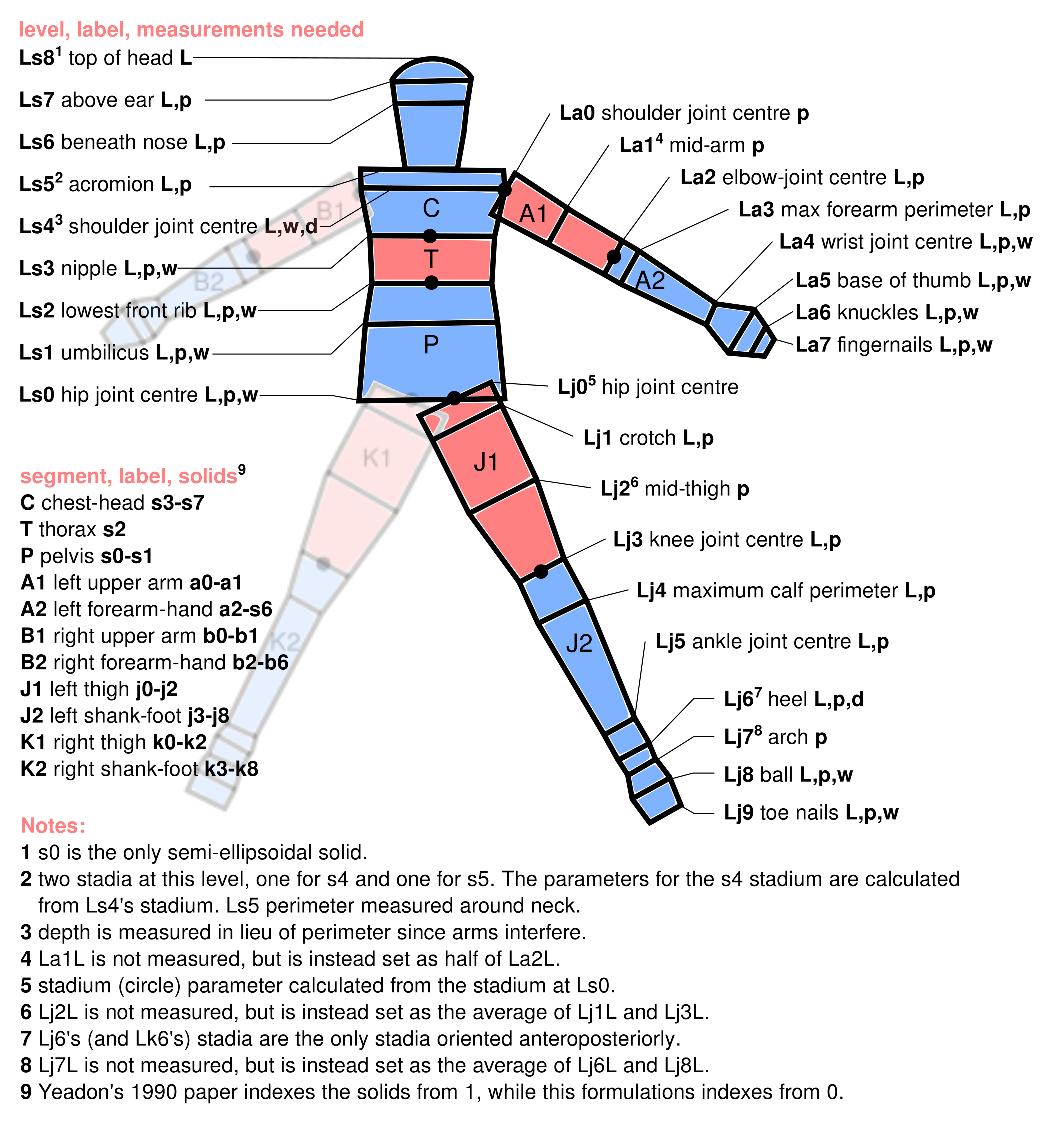
\includegraphics{measurements.eps}
\end{center}
\caption{
{\bf Measurements required for the human inertia model.}  The human is defined
in terms of segments, levels, and solids. Segments are separated by alternating colors, and are denoted as \textbf{P},
\textbf{A1}, etc. Levels are denoted as ``\textbf{L$<$s$>$\#}'', where \textbf{$<$s$>$}
denotes a part of the body (e.g. \textbf{j} for the left leg) and \textbf{\#}
denotes the index of the level in the part of the body. The solid ``above''
level \textbf{L$<$s$>$\#} is denoted as ``\textbf{$<$s$>$\#}''. The model is
personalized via 95 measurements, of which there are 4 types: lengths
\textbf{L} along the longitudinal axis of the segments, perimeters \textbf{p}
about the segments, mediolateral widths \textbf{w}, and anteroposterior depths
\textbf{d}. Black dots denote joint centers \cite{Yeadon1990c}.
}
\label{fig:meas}
\end{figure}

\begin{figure}[!ht]
\begin{center}
%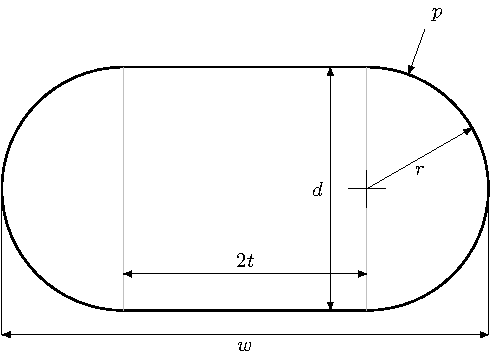
\includegraphics[width=3.27in]{stadium.tiff}
\end{center}
\caption{
{\bf Stadium cross section shape.}  The levels that define the segments are all
in the shape of a stadium, with one exception. We can define a stadium by
by any two of its attributes: perimeter $p$, radius $r$, thickness $t$,  width
$w$, and depth $d$.
}
\label{fig:stadium}
\end{figure}

\begin{figure}[!ht]
\begin{center}
%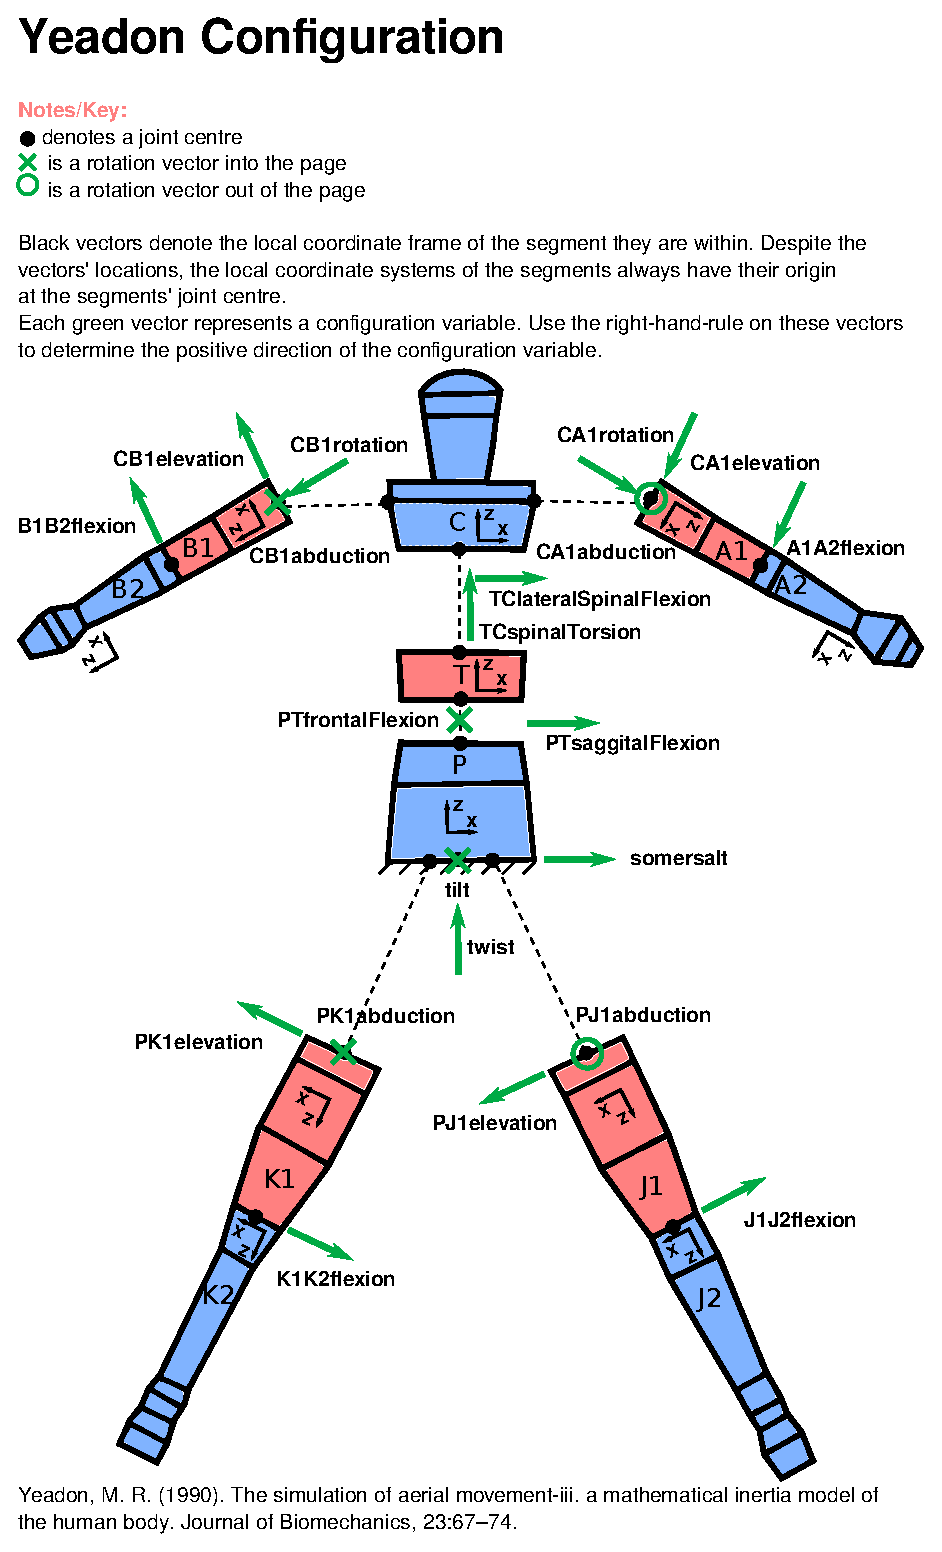
\includegraphics{configuration.eps}
\end{center}
\caption{
{\bf Configuration variables for the human inertia model.}  The configuration
of the human is defined using 21 joint angles, represented by green vectors. A
green cross represents a vector into the page, and a
green circle represents a vector out of the page. The direction of rotation for
a joint angle is given by the right-hand rule about its vector. The labels
beside the vectors are the names of the configuration variables in the code.
The black dot on each segment denotes its joint center. The origin of the
global fixed coordinate frame is at the bottom center of the
pelvis segment. The local coordinate frame of each segment is specified by the
pair of perpendicular black vectors in or next to the segments. Despite the
locations of these black vectors, the origin of a segment's local coordinate
system is always at its joint center \cite{Yeadon1990e}.
}
\label{fig:config}
\end{figure}

\begin{figure}[!ht]
\begin{center}
%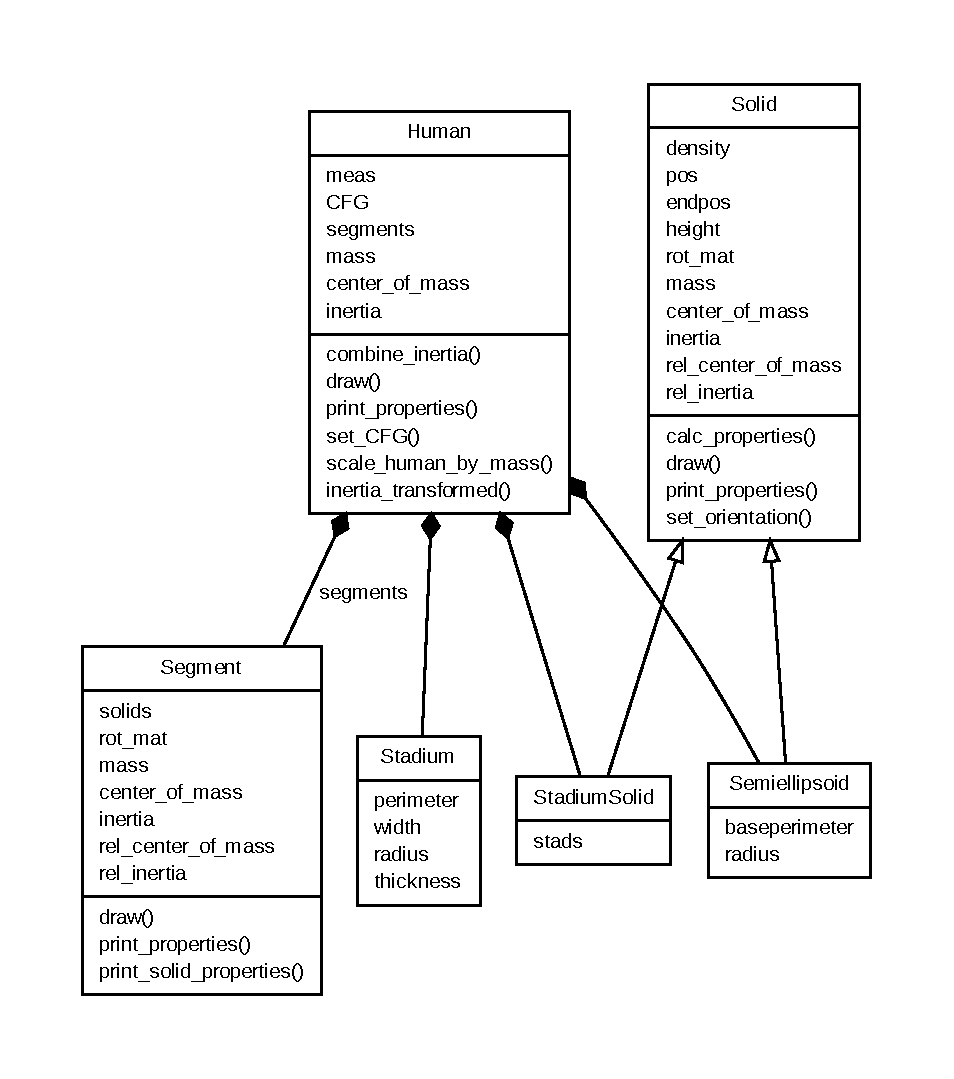
\includegraphics{umldiagram.eps}
\end{center}
\caption{
{\bf UML diagram of Yeadon package.}  The Human class constructs all
Segment's, Solid's, and Stadium's, and assembles them
appropriately. The classes StadiumSolid and Semiellipsoid inherit
from Solid. This diagram does not reveal the entire public interface of
the classes shown. The user interacts with module through the attributes or
methods of the Human class, or via the ui or gui modules.
}
\label{fig:umldiagram}
\end{figure}

\begin{figure}[!ht]
\begin{center}
    \missingfigure{iceskater}
%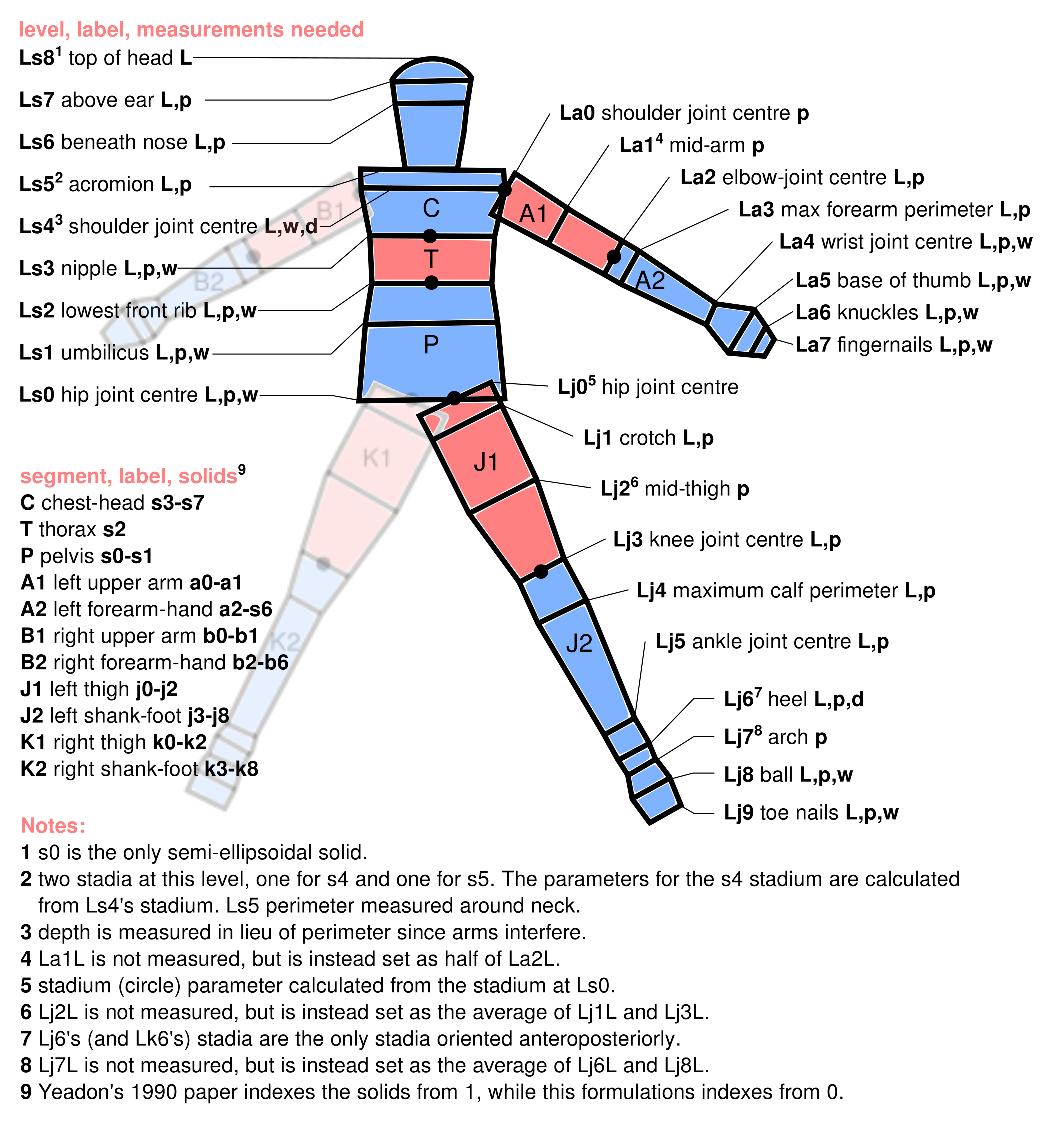
\includegraphics[width=4in]{measurements.eps}
\end{center}
\caption{
{\bf TODO Bold the first sentence.}  Rest of figure 2  caption.  Caption 
should be left justified, as specified by the options to the caption 
package.
}
\label{fig:iceskater}
\end{figure}

\section*{Tables}
%\begin{table}[!ht]
%\caption{
%\bf{Table title}}
%\begin{tabular}{|c|c|c|}
%table information
%\end{tabular}
%\begin{flushleft}Table caption
%\end{flushleft}
%\label{tab:label}
% \end{table}

\begin{table}[!ht]
\caption{
\bf{Length measurements}}
\begin{tabular}{|c|c|}
    \hline
    \textbf{length for these levels} & \textbf{are measured from this level}\\
    \hline
    Ls1 - Ls5 & Ls0 \\
    \hline
    Ls6 - Ls8 & Ls5 \\
    \hline
    La2 - La4 & La0 \\
    \hline
    La5 - La7 & La4 \\
    \hline
    Lb2 - Lb4 & Lb0 \\
    \hline
    Lb5 - Lb7 & Lb4 \\
    \hline
    Lj1, Lj3 - Lj5 & Lj0 \\
    \hline
    Lj8 - Lj9 & Lj5  \\
    \hline
    Lk1, Lk3 - Lk5 & Lk0 \\
    \hline
    Lk8 - Lk9 & Lk5  \\
    \hline
\end{tabular}
\begin{flushleft}The length measurements are not simply the heights of the
    stadium solids. They are defined relative to a certain preceding level in
    their segment.
\end{flushleft}
\label{tab:length}
\end{table}

\begin{table}[!ht]
\caption{
\bf{Rotation order for multi-degree of freedom joints}}
\begin{tabular}{|c|c|}
    \hline
    \textbf{joint(s)} & \textbf{order of rotations}\\
    \hline
    P & somersalt, tilt, twist \\
    \hline
    PT & frontal flexion, sagittal flexion \\
    \hline
    TC & torsion, lateral spinal flexion \\
    \hline
    CA1, CB1 & elevation, abduction, rotation \\
    \hline
    PJ1, PK1 & abduction, flexion \\
    \hline
\end{tabular}
\begin{flushleft}Since rotations are not commutative, we must specify the order
    in which we perform rotations at multi-degree of freedom joints. For each
    joint with more than one configuration variable, we provide the order in
    which we rotate the segment with respect to the orientation of the
    preceding segment.
\end{flushleft}
\label{tab:dof}
\end{table}


\end{document}
